%!TEX root = ../dissertation.tex

\begin{savequote}[75mm]
Another inspiring quote for this chapter
\qauthor{Another author maybe}
\end{savequote}


\chapter[Improving the Speed and Quality of Cancer Segmentation Using Lower Resolution Pathology Images]{Improving the Speed and Quality of Cancer Segmentation Using Lower Resolution Pathology Images}
 
\lettrine[lines=3]{\textcolor{SchoolColor}{I}}{n this paper},
we propose a pipeline to investigate the performance of semantic segmentation model that employs an encoder-decoder architecture with atrous separable convolution and spatial pyramid pooling, trained on multi-resolution whole slide breast pathological images with different patch sizes. Our segmentation model obtains the best performance on zoom level 2 (10$\times$magnification) with AUC score 0.974 in terms of slide-level classification. This outperforms both the performance of the pathologist and other semantic segmentation models on the Camelyon16 dataset. By offering a larger field of view and reducing noise and detail, training
a semantic segmentation model on the properly selected lower resolution pathology images can further improve the precision of pixel-wise cancer region segmentation. By contrast, the corresponding inference time is 14 times shorter than the inference time trained on the highest resolution patches, and it is also shorter than the time required by a pathologist with time constraints.
Moreover, we prove that the model trained on lower resolution patches can still generate refined external polygons of cancer region on the highest resolution image. This study provides new insights into efficient gigapixel histopathology analysis that will make clinical adoption more likely.

\section{Introduction}\label{se:3-1}

As the highest incidence rate of cancer among women and the second leading cause of cancer death worldwide, breast cancer can be seen nowadays as the most serious threat to women's health. In 2019, 111,710 new cases of breast cancer were diagnosed worldwide and 41,760 woman died from it~\cite{Siegel2019}. However, with the development of pathology instrumentation and accessories, standardized pathological examination  can essentially contribute to better diagnosis and treatment of breast cancer. Especially in recent years, the possibility to capture an entire slide and save it in a digital format named Whole-Slide Image (WSI) enables pathologists to examine the biopsy at different levels of magnification, which significantly increased the accuracy of diagnosis~\cite{Pantanowitz2010}.  

However, manual microscope image examination is a time-consuming and tedious task and is made more difficult by the fact that tumor cells often occur as small patches that are difficult to spot. Computer-assisted pathology image analysis is therefore needed to help pathologists detect small metastatic areas in a more accurate and efficient manner. Machine learning has been widely adopted in the computer vision domain~\cite{khan2020machine,voulodimos2018deep,liu2020reliability}. For example, deep learning models and, particularly, Convolutional Neural Networks (CNNs), have been extensively utilized in medical image analysis~\cite{liu2021medical,liu2021review,Hou2016,Li2018,wang2021tumor,Deepa2022,gupta2022deep,singh2022breast,murtaza2020breast,chanchal2022deep}. In order to obtain better model accuracy, the number of parameters that need to be trained has dramatically increased, as CNN architectures go wider and deeper. However, training such models has significantly higher computation and memory demands. Hence, High Performance Computing (HPC) facilities based on CPU~\cite{codreanu2018}, GPU~\cite{Wang2022} and FPGA~\cite{Geng2018} enable training such heavy models while significantly reducing training times, which also benefits the WSI analysis.

The WSIs are typically high resolution images with a relatively large memory footprint. The size of one WSI could be around 2 gigabytes (GB) considering the slide image dimensions of 200,000 by 100,000 pixels in the highest resolution mode ($40\times$ magnification). However, since loading an entire WSI is currently still computationally intractable~\cite{Komura2018}, a typical approach to tackle this challenge is to extract smaller, manageable
patches from the highest resolution WSI and perform binary classification training and prediction of tumors by using deep convolutional neural network methods~\cite{Wang2016,Li2018}.

The Cancer Metastases in Lymph Nodes Challenge 2016 (i.e. CAMELYON16 or Camelyon16) was initiated by the IEEE International Symposium on Biomedical Imaging (ISBI) with the aim of detecting the presence of breast cancer metastases in lymph nodes~\cite{Bejnordi2017}. It has since become one of the most widely-used public datasets for studying cancer detection using deep learning methods~\cite{Wang2016,Liu2017,zhang2023whole,shen2022identify,yu2023bayesian,tourniaire2023ms,khaliliboroujeni2022end,jin2020integrative,liu2020effidiag,Guo2019}. The work presented in~\cite{Wang2016}, which won the Camelyon16 challenge~\cite{Bejnordi2017} with patches size $256\times256$ using GoogLeNet architecture~\cite{Szegedy2015}, reports the best results on the highest zoom level ($40\times$) images. However, this conclusion is based on patch-level classification, which has several limitations. Firstly, since the approach of patch level classification is predicting the whole patch as positive or negative, it ignores the situation where tumor and healthy tissue are coexisting in the same patch and can only generate prediction on very low resolution masks~\cite{Liu2017}. Secondly, in order to create relatively dense heatmap predictions, they have to extract relatively small patches such as $256\times256$ and $299\times299$ from the highest resolution ~\cite{Liu2017,Wang2016} . Such small patches on the highest resolution can not provide sufficient contextual information, which may lead to inconsistent predictions. Thus, there is a contradiction between patch size and dense prediction by using patch level classification methods. Some attempts have been made to consider the spatial correlations of neighboring patches such as introducing Conditional Random Field (CRF)~\cite{Li2018}. This has only been tested on small numbers of neighboring patches so the contextual information that can be learned is still limited. Finally, the number of patches extracted from single WSI would be around 10,000 to 400,000 (median 90,000)~\cite{Liu2017}, which is very time consuming and computationally intensive in terms of data preprocessing and prediction. 

In contrast, semantic segmentation models can generate refined predictions by performing pixel-level classification and do not need to consider the trade-off between patch size and prediction quality. In recent years, several attempts have been made to investigate the training of semantic segmentation models on the highest resolution WSI such as~\cite{Guo2019}. However, the performance of the model with the largest patch size $1024\times1024$ (AUC 0.95) reported from the paper is still lower than that of the pathologist without time constraints (AUC 0.966) with relatively long inference time (79~mins/slide) using one GTX 1080Ti GPU, which may hinder clinical adoption. Using similar-sized patches extracted from lower resolution WSI offers a larger field-of-view (FoV), since the amount of extracted patches for prediction is significantly smaller compared to the highest resolution one. This may contribute to better model performance and shorter inference time. Therefore, it is worth investigating the performance of semantic segmentation models on different zoom levels using HPC resources, as this facilitates pixel-wise classification instead of patch level classification.  

In this paper, we introduce a framework to evaluate the performance of a semantic segmentation model (DeepLabV3+) on various lower zoom levels, comparing them to the highest resolution patches ($40\times$ magnification), to explore the feasibility of training deep convolutional neural network with lower resolution images. We also conduct a comparison of model performance among different patch sizes trained on lower resolution. To our knowledge, no research has focused primarily on the trade-off between different zoom levels, segmentation models performance, and corresponding training and prediction time, which would offer insight into efficient gigapixel histopathology image analysis and its potential for clinical adoption.

The main contributions of this work are the following:

\begin{itemize}
\item Properly selecting lower resolution pathology images ($10\times$ magnification) can contribute to better semantic segmentation model training and prediction. It overcomes the limitation of patch-level classification using the highest resolution WSI, which generates low-resolution predictions by predicting the whole patch as positive or negative and ignoring coexisting tumor and healthy tissue within the same patch.
\item The semantic segmentation pipeline we proposed succeeds in outperforming pathologists. Additionally, the inference time is 14 times shorter than both the model trained on the highest resolution patches, and is also shorter than the time required by pathologists with time constraints.
\item Our model, trained on lower resolution patches ($10\times$ magnification), generates more precise segmentation than the same model trained on higher resolution patches. It accurately produces external boundaries of cancer regions on the highest resolution image ($40\times$ magnification), indicating its potential as a computer-assisted diagnostic and annotation tool to help pathologists reduce labeling time and identify cancerous regions.
\end{itemize}

\section{Dataset and evaluation metrics}\label{se:3-2}

To compare our workflow with state-of-the-art strategies, as a testbed for this study we adopt well-known Camelyon16 dataset, a publicly available WSI dataset of lymph node section~\cite{Bejnordi2017}. We further adopt the evaluation strategy from the Camelyon16 challenges with regard to  slide-level classification. The details are discussed in the following subsections.

\subsection{Camelyon16 dataset}\label{se:3-2.1}

The Camelyon16 dataset has 270 pixel-annotated WSIs obtained from the sentinel lymph nodes of breast cancer patients. The objective of the competition is to develop an algorithm capable of automatically detecting the scope of breast cancer metastasis in lymph node slices stained with Hematoxylin and Eosin (H\&E). These contain 110 metastases collected in the Radboud University Medical Center and the University Medical Center Utrecht. The average memory footprint of a WSI in the Camelyon16 dataset is around 1.9 GB, with the smallest WSI being 522MB and the largest 3.8GB. At the highest magnification level, WSIs have an average width of 109,666 pixels, ranging from 45,050 to 221,184 pixels, and an average height of 173,012 pixels, ranging from 28,672 to 221,696 pixels. The WSIs are stored in a 3-channel encoded TIFF format, which involves multiple levels of downsampling, to address the different zoom levels in one image. The largest resolution can be obtained at $40\times$ magnification, which is also considered level 0, while the magnification of $20\times$ corresponds to level 1, $10\times$ corresponds to level 2 etc.

\subsection{Evaluation metrics}\label{se:3-2.2}

In this study, we use the first evaluation strategy (i.e. Slide-based Evaluation) of the Camelyon16 challenge to measure the performance of our predictions\footnote[1]{https://camelyon16.grand-challenge.org/Evaluation/}. It enables us to compare our model results with the Public Leaderboard 1 in Camelyon16 challenge in terms of WSI classification task. This metric evaluates the performance of classification models at discriminating between WSIs which contain metastasis and normal slides. In the challenge, participants submit the list of probabilities which indicate the likelihood of each slide containing tumor and the area under the receiver operator curve (AUC) will be calculated to measure the performance of the model~\cite{Bradley1997}. We use percentile bootstrap method and construct 95\% confidence intervals for AUC score calculation~\cite{Efron1979}.

\section{Method}\label{se:3-3}

In this section, we further describe the testbed used for our study, including the complete proposed workflow, model details, and hardware configuration. Figure~\ref{fig:3-1} illustrates  the cancer metastasis detection workflow in our study, which can be divided into training and prediction pipelines. The training pipeline encompasses patch extraction from WSI tissue areas with multiple magnification levels and corresponding DeeplabV3+ model training. The prediction pipeline involves patch extraction, inference, pixel-wise tumor probability heatmap generation, cancer regions segmentation, and slide-based classification. The details are explained in the following subsections.

\begin{figure}[!ht]
\centering
\includegraphics[width=0.9\textwidth]{3-1.eps}
\caption{Overview of the proposed pipeline.}
\label{fig:3-1}
\end{figure}

\subsection{Data preprocessing}\label{se:3-3.1}

In this section, we describe how we removed the background area from the whole-slide images (WSI) to extract only the tissue area and generate non-overlapping patches. We also outline our data preparation and augmentation steps for model training. The details are discussed in the following subsections.

\subsubsection{Patch sampling}\label{se:3-3.1.1}

In our data preprocessing pipeline, we use Openslide~\cite{GOODE201327}, a C library that provides a simple interface for reading whole-slide images, to open the Camelyon16 pathology image files. To prevent generating many white (empty) patches, similar to~\cite{khened2021generalized} and inspired by Otsu's seminal work~\cite{4310076}, we convert WSIs from BGR to HSV color-space and threshold the three channels of HSV image in the range of 0 to 200 to obtain the tissue area,  We then perform morphological open and closing operations to eliminate any noise present. Next, we use the \texttt{cv2.findContours} and \texttt{cv2.boundingRect} functions to generate contours of the areas containing cell tissues and to draw a bounding box outside the contours in preparation for the patch extraction process. Subsequently, we extract non-overlapping patches of size ($768\times768$) using sliding windows inside the bounding boxes of these contours only. After generating a patch, a post-processing step is performed looking at the standard deviation of the patch in combination with the amount of black and white pixels, to investigate whether pixels in the patch are part of the artefacts in the background (e.g. some WSI's have black background). If that is the case, the patch is discarded. Using the same method, we extract the tissue area, calculate the percentage of tissue in each patch, and conduct the sampling as follows. For negative patch sampling, i.e. sampling of patches that do not contain any cancerous tissue, we only extract negative patches from normal WSI to avoid the interference of rough annotation. In addition, we select patches which contain more than 5\% tissue area. As for positive patch sampling, patches containing more than 0.5\% cancer area from tumor WSI are considered as positive patches. The ratio of positive and negative patches used for training is 1:3, which is different from some related work, such as~\cite{Lee2018,Li2018}, that sample the same number of tumor and normal patches. The reason for increasing the ratio of negative patches in the training set is the following: unlike patch-level classification, semantic segmentation models enable more precise prediction but also significantly increase the chance of wrong predictions, and in particular false positives, since they perform pixel level classification. Such wrong predictions will highly impact the WSI classification results. Contrary to balancing the classes by performing under-sampling of the majority category as in~\cite{Lee2018,Li2018}, we conjecture that a higher ratio of negative patches will allow the model to better capture variety in the data by avoiding loss of potentially useful information. We confirm this assumption empirically by obtaining a higher WSI classification accuracy when training the model with ratio 1:3 instead of 1:1.

\subsubsection{Patch augmentation}\label{se:3-3.1.2}

Since the slides of Camelyon16 are collected from two medical centers, staining variability is often present in the training dataset, which may be caused by different product of hematoxylin and eosin-stains or subtle difference in chemical staining procedures. Several publications indicate high staining variations will negatively affect the model performance~\cite{Lee2018,Dimitriou2019}. In general, there are two approaches to tackle this problem. The first approach is to implement stain-color normalization~\cite{Magee2009,Zanjani2018}. The second approach is to force the model to ignore the color variation in patches by adopting hard color augmentation~\cite{xu2020colorectal,wu2022machine}. 
In order to force the model to ignore staining variability, we adopt hard data augmentation due to the time-consuming nature of stain color normalization, which needs to be implemented during both the training and inference processes. We apply random hue, saturation, brightness and contrast as described in Table~\ref{tab:3-1}. In addition, we also add random flip to our data augmentation process.

\begin{table}[!h]
\centering
\caption{Patch augmentation details.}
\label{tab:3-1}
\setlength{\tabcolsep}{1.8mm}{
\begin{tabular}{lll}
\toprule
\textbf{Methods} & \textbf{Details} & \textbf{Triggering Probability} \\ 
\midrule
Random Hue & maximum delta of 0.2 & 0.66 \\
Random Saturation & random saturation factor in [0.5, 1.5] & 0.66 \\
Random Brightness & maximum delta of 0.5 & 0.66 \\
Random Contrast & random contrast factor in [0.7, 1.3] & 0.66 \\
Flip & Left/right flip & 0.66 \\ 
\bottomrule
\end{tabular}}
\end{table}

\subsection{Semantic segmentation model}\label{se:3-3.2}

For the semantic segmentation task we use the DeeplabV3+ architecture developed by Google~\cite{Chen2018}, which proved to be highly effective in semantic segmentation tasks on the benchmark datasets, such as PASCAL VOC 2012~\cite{Everingham2015} and Cityscapes~\cite{Cordts2016}. DeeplabV3+ architecture is shown in Figure~\ref{fig:3-2}.The whole network can be considered as an Encoder-Decoder structure. For the encoder part, it mainly uses the architecture proposed in the DeeplabV3 paper~\cite{Chen2017}, which includes dilated convolutional operators and Atrous Spatial Pyramid Pooling (ASPP) capable of extracting features at different scales of receptive fields. To ensure that the memory footprint of the activation maps and therefore model remains within the hardware boundaries, this scaling is done by dilating convolutional operators. The multi-scale traits of the architecture fit the hypothesis about achieving better tumor segmentation by enlarging the patch size, thus taking in account more information due to the larger scale. The formal definition of the atrous convolution operation on the input feature map $x$ is given in Equation~\eqref{eq:multiscale}. Here $f_{i}$ is the output feature map $f$ at location $i$, $\mathbf{c}$ is the convolutional filter with length $\ell$ and the dilation rate $d$ determines the stride of the input $\mathbf{x}$~\cite{Chen2018}.

\begin{figure}[!ht]
\centering
\includegraphics[width=1.0\textwidth]{3-2.eps}
\caption{An overview of DeeplabV3+ architecture.}
\label{fig:3-2}
\end{figure}

The decoder part is for the first time introduced in DeeplabV3+ architecture. In the former generation of Deeplab model (DeeplabV3)~\cite{Chen2017}, the encoder generates the feature maps with output stride 16, bilinearly upsampled to the original patch size. However, this method is not effective in terms of obtaining detailed object boundaries. Therefore, the decoder first upsamples the feature map generated from the encoder by a factor of 4. It then concatenates this with the low-level features from the backbone with corresponding spatial resolution after $1 \times 1$ convolution. Subsequently, the merged feature map will be passed through another $3 \times 3$ convolution and upsampled again by a factor of 4 to the original input size.
\begin{equation}
f_{i}=\sum_{\ell=1}^{\ell} \mathbf{x}(i+d \cdot \ell) \mathbf{c}(\ell)
\label{eq:multiscale}
\end{equation}

In addition, DeeplabV3+ uses atrous separable convolution to reduce the computation complexity of the proposed model while maintaining similar (or better) performance. It performs atrous convolution operations on each channel of input features separately, followed by a pointwise convolution to combine the output from atrous depthwise convolutions across channels. In our training process, we loaded the pre-trained PASCAL-VOC 2012 weights on the Xception backbone~\cite{8099678}. The Xception backbone in DeeplabV3+ has been modified as follows: (1) More layers are added. (2) All max pooling layers have been replaced with depthwise separable convolutions with strides. (3) Batch normalization and ReLU activation were introduced after each $3 \times 3$ depthwise separable convolution.

\subsection{Pipeline of WSI prediction}\label{se:3-3.3}

In order to evaluate the performance of our model trained on multiple zoom levels and patch sizes, we set up the WSI prediction pipeline, which is also illustrated in the testing stage of Figure~\ref{fig:3-1}. Similar to patch sampling, non-overlapping patches from different zoom levels are sequentially extracted from the bounding boxes of tissue area and fed into the trained model for inference. For example, $768\times768$ patches extracted from level 1 are sent to model trained on level 1 and so on. In order to accelerate the inference process, for level 0 and 1, we predict the patches which contain more than 20\% tissue area in order to avoid irrelevant predictions on background or fat tissue. As for level 2 and level 4, since the extracted patches have a relatively large field of view (FoV), we reduce the threshold of tissue area from 20\% to 10\% in order to avoid missing tissue area during the patch prediction. Figure~\ref{fig:3-3} shows an example of $768\times768$ patches extracted from the test set from level 0 to 4. Note that the extracted patches cover the tissue area of WSI. Similar to \cite{Li2018}, the patch prediction will be resized to the corresponding size on level 6 and stitched on a level 6 blank mask for post-processing. Since semantic segmentation inevitably leads to false positives, we first list the top 50 pixels from the WSI prediction based on the metastasis probability in descending order. Then, the mean of tumor probabilities is calculated and used as the likelihood of containing cancer for a single WSI.

\begin{figure}[!h]
\centering
\includegraphics[width=0.7\textwidth]{3-3.eps}
\caption{Patches extracted for prediction from different zoom levels}
\label{fig:3-3}
\end{figure}

\subsection{Hardware configuration}\label{se:3-3.4}

The training exercise of this study was implemented on the GPU nodes from the LISA Compute Cluster at the Dutch National Supercomputing Centre SURFsara\footnote[2]{https://userinfo.surfsara.nl/systems/lisa/description}. The training with patch sizes from 384 to 1024 on each level is performed on two GPU nodes, each consisting of one Intel Xeon Gold 5118 Processor and four NVIDIA Titan RTX GPUs with 24 GB of GDDR6 memory. For the inference step, we still used NVIDIA Titan RTX GPU node but only one GPU was needed for prediction because the inference process is not very time consuming. Therefore, the figures of prediction time presented in Table~\ref{tab:3-3} are based on using a single NVIDIA Titan RTX GPU.

\section{Results}\label{se:3-4}

We conduct a series of experiments to answer the following research questions:
\begin{enumerate}
\item How does the model performance change when training with multi resolution pathology images? Is it possible to achieve even a better result at lower magnification levels?
\item Can such training protocol on WSIs yield a comparable performance to pathologist and state-of-the-art automatic approaches working with high-resolution images?
\item What is the difference in inference time between models trained on different WSI resolutions and pathologist performance?
\item Can the presented model trained with lower resolution images still generate refined external polygons of cancer region on the highest resolution?
\end{enumerate}

\subsection{Performance of the model trained on different zoom levels and patch sizes}\label{se:3-4.1}

The results of our model trained on different zoom levels and patch sizes performing the Camelyon16 WSI Classification task are shown in Figure \ref{fig:3-4}. The left part of the figure presents the ROC curves of DeeplabV3+ trained from zoom level 0 to 4 with same patch size $768\times768$. AUC indicates the area under the receiver operating characteristic curve. We observe that the model trained on level 2 patches achieves the best AUC score of 0.9713. The figure on the right demonstrates the classification performance of models trained with four different patch sizes (i.e. 384, 512, 768, and 1024) on level 2. The model trained on $1024\times1024$ patch size achieves the best result (0.9741), and we observed a general trend suggesting that larger patches lead to better model performance. In addition, interesting comparison between the model trained with $384\times384$ patches on level 2 and $768\times768$ patches on level 1 can be made because they contain the same FoV. The result shows that the model trained with $384\times384$ patches on level 2 achieves better results (0.9591) than $768\times768$ patches on level 1 (0.9564), which indicates that even in the condition of same FoV, the model trained on level 2 still gets better performance. 

\begin{figure}[!h]
\centering
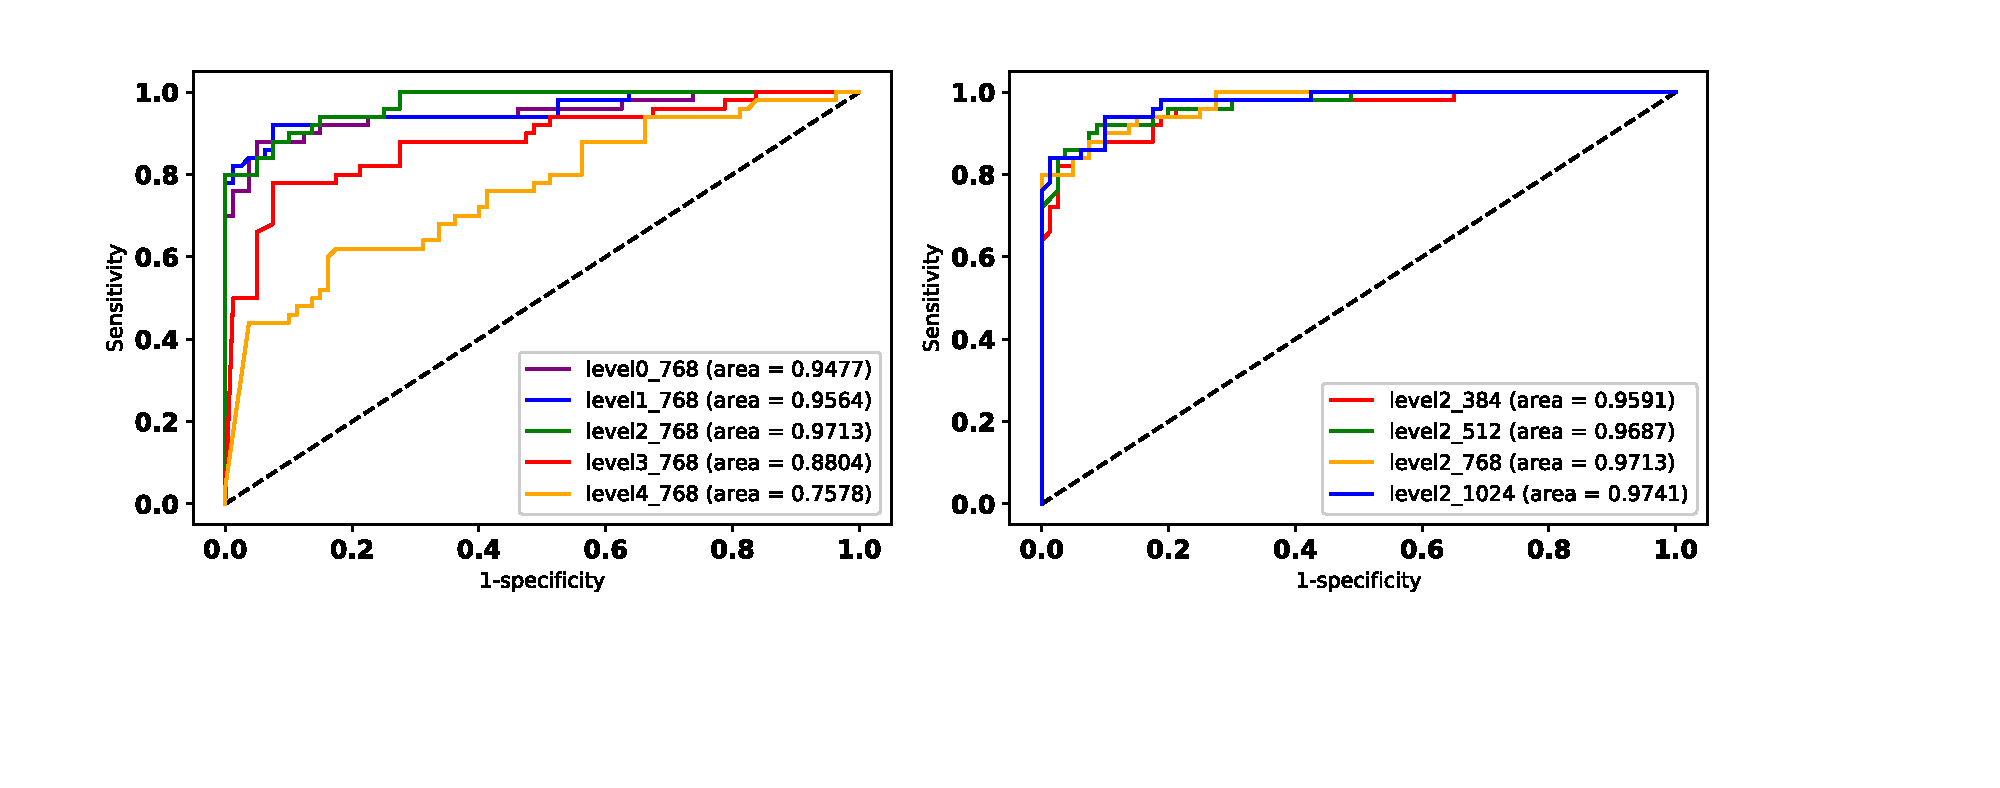
\includegraphics[width=0.95\textwidth,trim = 10 70 10 20, clip]{3-4.eps}
\caption{Comparison results of our models trained on different zoom levels
and patch sizes}
\label{fig:3-4}
\end{figure}

Figure \ref{fig:3-5} illustrates the comparison between our model trained on multiple zoom levels with a patch size of $768\times768$ pixels and the performance of pathologists, both without time constraints (WOTC) and with time constraints (WTC)~\cite{Bejnordi2017}. It firstly shows a clear trend on how model performance changes with the increasing zoom levels. Namely, the model performance improves in the WSI classification task when the zoom level increases from 0 to 2, but dramatically drops at levels 3 and 4. We assume that the reason for lower performance on zoom levels 3 and 4 lies in excessive down-sampling loses, which make it for the segmentation models very hard to distinguish tumor area from normal tissue. In addition, our model trained on zoom level 2 achieves better results than the pathologist WOTC.
\begin{figure}[!h]
\centering
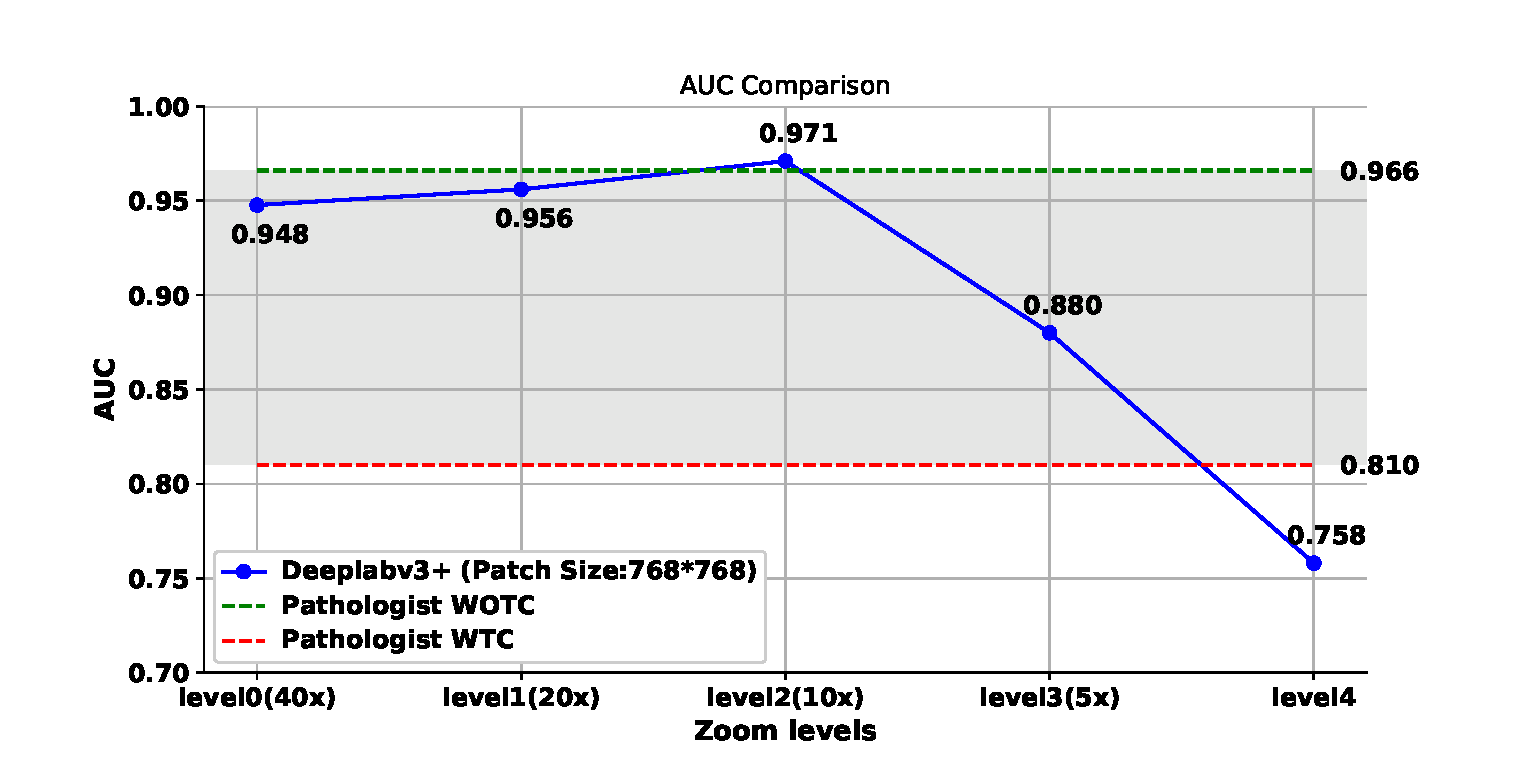
\includegraphics[width=0.9\textwidth]{3-5.eps}
\caption{Comparison results of our methods with pathologist performance}
\label{fig:3-5}
\end{figure}

\subsection{Comparison with state-of-the-art}\label{se:3-4.2}

In addition, we compared our results with the official leaderboard of the Camelyon16 challenge and state-of-the-art papers using Camelyon16 dataset (Table \ref{tab:3-2}). Our pipeline based on DeeplabV3+ model trained with $1024\times1024$ patches on level 2, achieved third place in Whole-slide-image classification public Leaderboard 1 \cite{camelyon16}. It should be noted that a remarkable AUC score of 0.994 can be achieved by employing additional computationally demanding procedures, such as stain normalization and a smaller inference stride. However, this outcome is less noteworthy and presents considerable obstacles to clinical implementation due to the substantially increased computational expense. Ideally, the diagnostic process should be executed promptly with minimal resource utilization. Since 2019, several papers studied the performance of more recent segmentation models on Camelyon16 dataset. The study presented in \cite{jin2020integrative} used ConcatNet (Four U-nets based on four histological features) and achieved an overall AUC 0.924. Another study \cite{Liu2017} applied Unet and EffiNet, yielding an overall AUC of 0.935. The research presented in \cite{Guo2019} implemented a classification model Inception-v3, followed by the use of a semantic segmentation model DCNN for enhanced segmentation, leading to an overall AUC of 0.966. However, those results didn't exceed the pathologist performance WOTC. Our model trained on level 2 patches obtained the best result (AUC 0.9742) for semantic segmentation on Camelyon16 dataset in terms of WSI classification task. 

\begin{table}[!h]
\centering
\caption{Comparison of the results obtained by our model trained on different zoom levels and state-of-the-art methods; we make a distinction between patch level classification and semantic segmentation prediction approaches}
\label{tab1}
\label{tab:3-2}
\setlength{\tabcolsep}{0.8mm}{
\begin{tabular}{p{3cm}p{4.8cm}p{3.67cm}p{0.9cm}}
\toprule
Author & Method & Prediction method & AUC \\
\midrule
Pathologist~\cite{Bejnordi2017} & N/A& N/A & 0.966 \\ 
Wang et al.~\cite{Wang2016}  & GoogLeNet& Patch level classification& \textbf{0.994} \\ 
Liu et al.~\cite{Liu2017} & ResNet & Patch level classification& 0.976\\
Zhang et al.~\cite{zhang2023whole} & DPN, Swin-Transformer, SVM & Patch level classification& 0.961\\
\multirow{2}*{Shen et al.~\cite{shen2022identify}} & Pathology Deformable Conditional Random Field & \multirow{2}*{Patch level classification} & \multirow{2}*{0.920}\\ 
Yu et al.~\cite{yu2023bayesian}  & Bayesian
Collaborative Learning & Patch level classification & 0.956\\
Tourniaire~et~al. \cite{tourniaire2023ms} & Mixedly Supervised-CLAM & Patch level classification & 0.982\\
Khaliliboroujeni et~al.~\cite{khaliliboroujeni2022end}  & ResNet50, spatial 
 and channel attentions & \multirow{2}*{Patch level classification} & \multirow{2}*{0.970}\\
\midrule
Quincy Wong~\cite{Bejnordi2017}  & SegNet & Semantic Segmentation & 0.865  \\ 
Jin et al.~\cite{jin2020integrative} & ConcatNet & Semantic Segmentation & 0.924 \\ 
\multirow{2}*{Liu et al.~\cite{liu2020effidiag}}  & \multirow{2}*{Unet, EffiNet} & Semantic Segmentation\! + Patch level classification & \multirow{2}*{0.935}\\
\multirow{2}*{Guo et al.~\cite{Guo2019}}  & \multirow{2}*{v3\_DCNN\_1280 (level0)} & Patch level classification +\!\!~Semantic Segmentation & \multirow{2}*{0.966}\\  
Our method& DeeplabV3+\_1024\! (level2) & Semantic Segmentation & \textbf{0.974} \\ 
Our method& DeeplabV3+\_768 (level2) & Semantic Segmentation & 0.971\\ 
Our method& DeeplabV3+\_512 (level2) & Semantic Segmentation & 0.969\\
\bottomrule
\end{tabular}}
\end{table}

\subsection{Training and prediction time comparison}\label{se:3-4.3}

Next to prediction accuracy, another important factor influencing clinical adoption is the average inference time on a single WSI. We only use one NVIDIA Titan RTX GPU to perform inference. Table \ref{tab:3-3} shows the Training and inference time comparison among our models trained on multiple zoom levels and patch sizes. The model trained on level 2 with a patch size of $1024\times1024$ has the shortest inference time (42 s per slide), which is lower than that needed by a pathologist WTC (56 s per slide)~\cite{Bejnordi2017}. This is because the number of patches extracted from lower resolution WSI for prediction is much lower than in case of the highest resolution. Based on the experimental results above, we propose that zoom level 2 ($10\times$ magnification) would be the appropriate magnification level to perform semantic segmentation on.

\begin{table}[!h]
\centering
\caption{Training and prediction time comparison of our models trained on different zoom levels and patch sizes}
\label{tab:3-3}
\setlength{\tabcolsep}{0.9mm}{
\begin{tabular}{lp{0.11\textwidth}p{0.07\textwidth}lp{0.10\textwidth}p{0.12\textwidth}p{0.14\textwidth}}
\toprule
Zoom level & Training set size & Batch size & Iterations & Training (h) & Prediction (h) & Prediction/ slide (m) \\ 
\midrule
{level 0($768\times768$)} & {56,632}& {4}& {25,000}& {10.12}& {21.31} & 9.83 \\
{level 1($768\times768$)} & {34,524}& {4}& {25,000}& {9.72} & {4.75}& 2.19 \\ 
\midrule
{level 2($1024\times1024$)} & {8,494}& {2}& {50,000}& {28.42} & {1.52}& {\textbf{0.70}}\\
{level 2($768\times768$)} & {10,420}& {4}& {25,000}& {9.58} & {1.55}& 0.71\\
{level 2($512\times512$)} & {23,256}& {4}& {25,000}& {6.2}& {2.12}& 0.97 \\
{level 2($384\times384$)} & {37,688}& {4}& {25,000}& {4.92} & {3.1} & 1.43 \\ 
\midrule
{level 3($768\times768$)} & {4,184} & {4}& {25,000}& {9.96} & {0.58}& 0.26 \\
{level 4($768\times768$)} & {1,992} & {4}& {25,000}& {9.23} & {0.23}& 0.18 \\ 
\bottomrule
 & & & & &&\\ 
\cmidrule{1-4}
\multicolumn{4}{l}{Pathologist WOTC: 13.95 m/slide}&&& 
\\
\multicolumn{4}{l}{Pathologist WTC: 0.93 m/slide} &&& \\ 
\cmidrule{1-4}
\end{tabular}}
\end{table}

\subsection{Segmentation result presentation}\label{se:3-4.4}

As we described previously, one of many advantages of performing semantic segmentation compared with patch-level classification is that it can offer refined cancer regions segmentation on high resolution WSIs, which can assist pathologists in identifying small metastasis area. This method could also be very useful when considered as a computer-aided annotation tool, which can significantly reduce the time of annotation for a pathologist. Therefore, it is worth evaluating the real segmentation performance of our model on both higher and lower resolution patches. In this study, we select our model trained on level 2 with a patch size of $768\times768$, as well as a model trained on level 1 with the same patch size, to generate binary predictions from heatmaps using a threshold of 0.5. Subsequently, we use \texttt{cv2.drawContours} function from OpenCV\footnote[3]{https://opencv-python-tutroals.readthedocs.io/} library to draw external polygons of cancer area. The segmentation result is shown in Figure \ref{fig:3-6}. Both models trained on level 1 and 2 can generate decent external polygons of the cancer area. However, we observe that the model trained on level 2 performs more precise segmentation than the one trained on level 1. The yellow arrows in Figure \ref{fig:3-6} show that some  subtle normal tissue and blank areas between tumor areas have been detected by the level 2 model but not by the level 1 one. In addition, several publications have discussed the issue of inaccurate labeling in histopathological imaging, including the Camelyon16 dataset~\cite{cheng2020self,gildenblat2019self,naouar2023robust}. Manually annotating large whole slide images on the pixel level of the highest magnification is an inherently challenging task, making it difficult to avoid unreliable labeling in practice. Notably, our model has the ability to accurately identify and label these areas. The fourth row of Figure~\ref{fig:3-6} illustrates an example in which some adipocytes were mistakenly labeled as tumors in the original mask, but our model trained on level 2 patches was able to accurately identify and correct them. Moreover, column (d) of Figure~\ref{fig:3-6} shows that even at the highest resolution, the polygons generated by our model trained on level 2 can still fit well with the tumor boundary, which indicates the interesting potential of our method in assisting pathologists with annotating high resolution images.

\begin{figure}[!h]
\centering
\includegraphics[width=0.9\textwidth]{3-6.eps}
\caption{External polygons of tumor regions generated by our models. From left to right, (a) is the prediction of model trained on level 2 shown at level 3 ($5\times$) patches, (b) is the prediction of model trained on level 1 shown at level 3 ($5\times$) patches, (c) is the Ground truth shown at level 3 ($5\times$), (d) is the prediction of model trained on level 2 shown at level 0 ($40\times$) patches, (e) is the ground truth shown at level 0 ($40\times$) patches.} 
\label{fig:3-6}
\end{figure}

We conjecture that the reason why the model on level 2 obtains the best result could be two-fold. Firstly, similar-sized patches extracted from lower resolution WSI offer a larger field-of-view (FoV), which contributes to better model performance in terms of segmentation and slide-level classification~\cite{Guo2019}. Secondly, although semantic segmentation models highly rely on the quality of annotation when performing supervised learning, it is nearly impossible for the pathologist to annotate pixel by pixel on the high resolution image. Therefore, training segmentation model on the highest magnification level would enable the model to obtain more details of tissue but at the same time, rough annotations also have a strongly negative impact on the performance of the model. Appropriate downsampling can makes the rough annotation on the highest resolution not obvious, therefore increasing the robustness of the segmentation model. Similar effect can be observed in using Gaussian filter to smooth the image and reduce the level of noise, which trades for better segmentation model performance~\cite{cai2017framework,nasor2021segmentation}. 

\section{Conclusion}\label{se:3-5}

In this paper, we study the impact of adopted resolution level and patch size on the performance of cancer region segmentation based on whole-slide images (WSIs) of sentinel lymph node. Firstly, we observe that the model achieves the best performance in the WSI classification task on zoom level 2 under the condition of same patch size and same field-of-view. Such results indicate that zoom level 2 (10$\times$) constitutes an appropriate magnification level for training and prediction of the semantic segmentation model in cancer metastasis detection. This interesting finding shows the possibility of efficiently training deep convolutional neural networks with lower resolution images. Secondly, the model trained on zoom level 2 patches achieved better performance than pathologist WOTC and, at same time, lower inference time than the pathologist WTC, which may help potential clinical adoption. Conclusively, our model trained on zoom level 2 patches can perform more precise segmentation than the same model trained on the higher-resolution patches, while still being able to generate refined external polygons of cancer regions on the highest resolution image. It indicates the potential of using these techniques as the basis for computer-aided annotation tools that help pathologists reduce the time taken by labeling. Further research on WSI analysis could include training models on zoom level 2 with even larger patch sizes, which can possibly lead to the training based on the entire WSI using more HPC capacity. The study could help identify the patch size for which the model performance becomes saturated and also show the limitations of current HPC facilities in terms of memory capacity. Moreover, it would be also interesting to explore the effects of using both data-parallelism and model parallelism strategies to process even larger patch sizes with the same model and hardware constraints.
